% IEEE standard conference template; to be used with:
%   spconf.sty  - LaTeX style file, and
%   IEEEbib.bst - IEEE bibliography style file.
% --------------------------------------------------------------------------

\documentclass[letterpaper]{article}
\usepackage{spconf,amsmath,amssymb,graphicx,epstopdf,url,float}
\usepackage{algpseudocode} 
\usepackage{algorithm}
\usepackage{mathtools}

\algnewcommand\algorithmicforeach{\textbf{for each}}
\algdef{S}[FOR]{ForEach}[1]{\algorithmicforeach\ #1\ \algorithmicdo}

\algdef{S}[FOR]{ForEachParallel}[1]{\algorithmicforeach\ #1\ \algorithmicdo \textbf{\ parallel} }

\algnewcommand{\LineComment}[1]{\State \(\triangleright\) #1}

\algnewcommand\True{\textbf{true}\space}
\algnewcommand\False{\textbf{false}\space}
\algnewcommand\Continue{\textbf{continue}\space}

% Example definitions.
% --------------------
% nice symbols for real and complex numbers
\newcommand{\R}[0]{\mathbb{R}}
\newcommand{\C}[0]{\mathbb{C}}

% bold paragraph titles
\newcommand{\mypar}[1]{{\bf #1.}}

% Title.
% ------
\title{Maximum Cardinality Matching for Bipartite Graphs}
%
% Single address.
% ---------------
\name{Thomas Meier, Isabelle Roesch, Conradin Roffler, Samuel Ueltschi} 
\address{Department of Computer Science\\ ETH Z\"urich\\Z\"urich, Switzerland}

\begin{document}
%\ninept
%
\maketitle
%

%The hard page limit is 6 pages in this style. Do not reduce font size
%or use other tricks to squeeze. This pdf is formatted in the American letter format, so the spacing may look a bit strange when printed out.

\begin{abstract}

Maximum cardinality matching, focus on existing algorithms and optimize the parallel versions in a highly multi-threaded environment. Focus on Pothen-Fan, reason about performance.

\end{abstract}

\section{Introduction}\label{sec:intro}

Matching in bipartite graphs has several applications in computer science, for example the marriage problem or computing the block triangular 
form (BTF) of a sparse matrix \cite{Pothen:1990}.\\

Two recent publications by Azad et.\ al.\ are concerned with solving the maximum cardinality matching problem in parallel. 
The first paper~\cite{Azad:2012} presents a parallel version of the Pothen-Algorithm (PPF) that achieves good performance 
on architectures with few fat cores. In the second paper a novel Parallel Tree Grafting (PTG) algorithm is presented 
that is designed to perform better on architectures with many thin cores. 
They also claim that PPF is not suited for architectures of this kind.\\

In this project we were able to recreate the result of the first paper (\cite{Azad:2012}) by writing an implementation of PPF
that matches the performance stated in the original paper. We give a detailed insight into our implementation and explain
implementation details and tricks that were omitted by the original authors of the algorithm. 
Furthermore we were able to improve upon the original algorithm by reducing the synchronization overhead of PPF (see section XY TODO ref).\\

We also implemented the PTG algorithm but were not able to reproduce the results of the original paper. 
Because we could not invest enough time to properly optimize the algorithm, we are not able to make any statements concerning this algorithm.
Nevertheless we give a brief introduction into PTG in section XY (TODO ref).\\

To verify the claim that PPF does not perform well on many thin cores, we conducted a series of experiments on the Xeon Phi platform~\cite{XeonPhi} (see section XY TODO ref). 
Our experiments show that PPF does in fact scale well on this platform by using our improvements to PPF. We also discovered that PPF
performs especially well when starting with a bad initial matching (see section XY TODO ref). 
By doing so we achieved superlinear speedup with PPF.

\section{Background: Algorithms for Maximum Matching in Bipartite Graphs}\label{sec:background}

\mypar{Maximum Cardinality Matching in Bipartite Graphs}
Given a bipartite graph $G = (V = X \cup Y, E)$.
A matching $M[\cdot]: |V| \rightarrow |V| \cup \{v_{null}\}$ is a mapping that assigns each node $v$ a unique mate $M[v]$ s.t. 
$\forall v \in V.\ M[v] \neq v_{null} \implies v = M[M[v]] \wedge \{v, M[v]\} \in E$.
Each vertex can have at most one mate. A vertex $v$ is matched if $M[v] \neq v_{null}$. An edge is matched if its vertices are matched. 
We call a matching a maximum cardinality matching if it maximizes the number of edges expressed by $M$. See~\cite{intro_alg} for a detailed introduction.

\mypar{Augmenting Path based Algorithms}
The algorithms presented in this report are based on augmenting paths. 
There are other classes of algorithms for this problem, namely push-relabel~\cite{GoldbergT88} and auction based~\cite{Bertsekas}. 
These however are not the focus of this report. 

The best known sequential algorithm for bipartite maximum cardinality matching was discovered by Hopcroft and Karp~\cite{HK:1973}
and runs in $O(|E|\cdot \sqrt{|V|})$. Another algorithm which runs in $O(|E|\cdot|V|)$ was discovered by Pothen and Fan~\cite{Pothen:1990}.
Although this algorithm asymptotically performs worse, in practice it performs better when parallelized according to Azad et.\ al.~\cite{Azad:2012}.

The core idea of both algorithm is to find so called augmenting paths. An augmenting path is a path where the edges alternate between matched an unmatched an where the first 
and last edge are unmatched. An augmenting path can be inverted by adding every unmatched edge to the matching and removing every matched edge from the matching. 
This will increase the size of the matching by one. 
Augmenting path based algorithms try to find and invert such paths. If there is no more augmenting path in a graph then the matching is maximal.

\mypar{Initial Matching}
Augmenting path based algorithms benefit from starting with an initial matching. 
A good algorithm for finding a good initial matching was discovered by Karp and Sipser~\cite{KarpS81}.
We use Karp-Sipser and an augmented greedy version based on Karp-Sipser to get an initial matching. 

\section{Algorithms and Optimizations}\label{sec:pfopt}

In this section, we describe how our PPF implementation works and how we optimized it. In addition to that, we 
give a brief theoretical analysis of PPF using the PRAM model. Furthermore we also discuss our Tree Grafting implementation.

\subsection{Parallel-Pothen-Fan}\label{sec:pf}

\mypar{Implementation}

Azad et.\ al.~\cite{Azad:2012} only give a very abstract description of their PPF implementation. In addition to that there is no source code available. 
Coming up with an efficient PPF implementation proofed to be challenging. 
In this section we describe our PPF implementation with a focus on the practical techniques we used to match the performance of performance Azad et.\ al.\\

PPF is computes the maximum cardinality matching by finding and inverting augmenting paths in parallel. 
A detailed explanation of the principles of PPF can be found in \cite{Azad:2012}. 
Our implementation is given in \texttt{PPF} (see algorithm~\ref{alg:ppf}). Functionally, the algorithm is equivalent to then one given by~\cite{Azad:2012} 
but goes into more detail and has some optimizations compared to the original.\\

The main loop iteratively performs multiple DFS searches in parallel to find augmenting paths. When a path is found, it is inverted to increase the matching.
This DFS search is given in the recursive algorithm \texttt{FIND\_AND\_AUGMENT} (see algorithm~\ref{alg:fa}). Our implementation of the DFS search finds a path and then inverts the matching while returning from the recursion. 
In practice, we used a stack based implementation of the recursive algorithm to avoid overflowing the stack as suggested by~\cite{Azad:2012}. 
Note that our algorithm only updates the matching of nodes on the right side of the graph. The left side can be updated later, when the algorithm is done. 
This saves unnecessary store instructions if an edge is added and removed from the matching multiple times.\\

Each thread has to lock the vertices it visits. The original PPF uses a $visited$ array of boolean flags to lock a vertex. 
All flags have to be reset after each iteration. This adds additional overhead because the resetting must be performed in the sequential phase of the algorithm.
We solve this problem by storing the current iteration number in the $visited$ array instead of just a flag when locking a vertex. The iteration number is increasing, 
therefore we know that a vertex is unvisited if the value in the $visited$ array is smaller than the current iteration. By using this technique, we do not have to clear
the visited array in each iteration which saves us $|Y|$ store instructions in the sequential phase of the algorithm.\\

Because all threads read and write the $visited$ array, all operations must be performed atomically to guarantee correctness because the algorithm. 
This is a large bottleneck of the algorithm because threads are blocked by waiting for the store operations of other threads to complete. 
In the original algorithm by Azad et.\ al.~\cite{Azad:2012}, Test-and-Set is used to claim the $visited$ array. 
An equivalent implementation of this approach in our algorithm is given in \texttt{$CLAIM_{TAS}$} (see algorithm~\ref{alg:claim_tas}). 
This is problematic however because Test-and-Set adds an unnecessary overhead to each failed attempt of claiming a vertex when there is no data race. 
We solved this issue by using the Test-and-Test-and-Set approach to lock vertices (see \texttt{$CLAIM_{TTAS}$} in algorithm~\ref{alg:claim_tas}).
Before using an atomic operation to lock a vertex, we first try a regular memory load. If the vertex is already locked we can omit the atomic operation. 
This has the benefit of increased caching an reduced memory traffic. We experimentally verified that Test-and-Test-and-Set performs better than Test-and-Set in section XY (TODO ref).

The source code of our PPF implementation is available online\footnote{\url{https://github.com/suem/dphpc-project}} for further details.\\

\begin{algorithm}
    \caption{Parallel Pothen Fan}
    \label{alg:ppf}
    \begin{algorithmic}[1]
        \Procedure{PPF}{$G=(V=X+Y,E), M$}

        \LineComment{Initialization}
        \State $lookahead[x] \gets \text{first neighbor of x}$ \Comment{$x \in X$}
        \State $iter \gets 0$
        \State $visited[y] \gets iter$ \Comment{$y \in Y$}
        \State $unmatched \gets \{x \in X, x \ \text{unmatched}\}$

        \LineComment{Discover augmenting paths}
        \Repeat 
            \State $iter \gets iter + 1$        
            \State $path\_found \gets \False$        
        \ForEachParallel{$x \in unmatched$}
            \If {$x$ matched}
                \State \Continue \Comment{skip $x$ if already matched}
            \EndIf
            \State $found \gets find\_and\_augment(x)$        
            \If {found}
                \State $path\_found \gets \True$        
            \EndIf
        \EndFor
        \Until{$path\_found = \False$}

        \LineComment{Complete matching}
        \ForEachParallel{$y \in Y$, $y$ matched}
            \State $M[M[y] \gets y$        
        \EndFor
        
        \EndProcedure
    \end{algorithmic}
\end{algorithm}


\begin{algorithm}
    \caption{Find and Augment}
    \label{alg:fa}
    \begin{algorithmic}[1]
        \Procedure{find\_and\_augment}{$x$}

            \LineComment{Lookahead Step}

            \ForEach{$y \in adj[x]$, starting at $lookahead[x]$}
                \State $lookahead[x] \gets \text{next neighbor of}\ x$
                \If {$y$ is unmatched}
                    \If {$claim(y)$}
                        \State $M[y] \gets x$ \Comment{make $x$ the mate of $y$}
                        \State \textbf{return} \True
                    \EndIf
                \EndIf
            \EndFor
            
            \LineComment{Recursive Path Search}
            \ForEach{$y \in adj[x]$}
                \If {$claim(y)$}
                    \State $success \gets find\_and\_augment(M[y])$
                    \If {$success$}
                        \State $M[y] \gets x$ \Comment{make $x$ the mate of $y$}
                        \State \textbf{return} \True
                    \EndIf
                \EndIf
            \EndFor
        \EndProcedure
    \end{algorithmic}
\end{algorithm}

\begin{algorithm}
    \caption{Claim with Test-and-Set}
    \label{alg:claim_tas}
    \begin{algorithmic}[1]
        \Procedure{$claim_{TAS}$}{$y$}
            \State $y\_iter \gets atomic\_exchange(visited[y], iter)$
            \State \textbf{return} $y\_iter < iter$
        \EndProcedure
    \end{algorithmic}
\end{algorithm}


\begin{algorithm}
    \caption{Claim with Test-and-Test-and-Set}
    \label{alg:claim_ttas}
    \begin{algorithmic}[1]
        \Procedure{$claim_{TTAS}$}{$y$}
            \If {$visited[y] < iter$}
                \State $y\_iter \gets atomic\_exchange(visited[y], iter)$
                \State \textbf{return} $y\_iter < iter$
            \EndIf
            \State \textbf{return} \False
        \EndProcedure
    \end{algorithmic}
\end{algorithm}

\mypar{PRAM Analysis}

The original authors of PPF did not provide a theoretical analysis of the runtime of the algorithm.
Doing such an analysis is non-trivial as the runtime of the algorithm mainly depends on the structure of the provided
input graph. If a graph has many non overlapping augmenting paths, then PPF performs well as there are no inter-thread conflicts. 
However if there are many overlaps then the threads will block each other often and the algorithm can only make little progress.
In this section we give a brief analysis of PPF using the PRAM model to illustrate the average parallelism of PPF for the best and worst case
scenario. \\

The work PPF has to perform is $O(|V|\cdot|E|)$. Finding an augmenting path requires a DFS of length at most $|E|$. 
This has to be performed for all $|V|$ vertices. Note that PPF might perform useless work that does not contribute to the solution
if it is blocked by another thread and has to abort the DFS. 
The PTG algorithm described in section XY (TODO ref) attempts to mitigate this problem.\\

Figure~\ref{fig:pram} illustrates the two program DAGs of PPF for the best case scenario (left) and the worst case (right).

In the best case scenario, the input graph only consists of non overlapping augmenting paths. 
Therefore all augmenting paths can be found in parallel. This is illustrated by the vertical gray node paths in the DAG.
Therefore the maximal depth of the DAG is $|E|$, the length of a DFS. Hence PPF as an average parallelism of $O(|V|)$ in the best case.\\

In the worst possible scenario, the input graph is consists of augmenting paths that always overlap. 
Therefore only one thread will succeed per operation and the other threads can't perform any work. This is indicated by the white nodes on
the DAG on the right. Therefore the depth of this DAG is the same as the work, yielding an average parallelism of $O(1)$.\\

\begin{figure}
    \begin{center}
  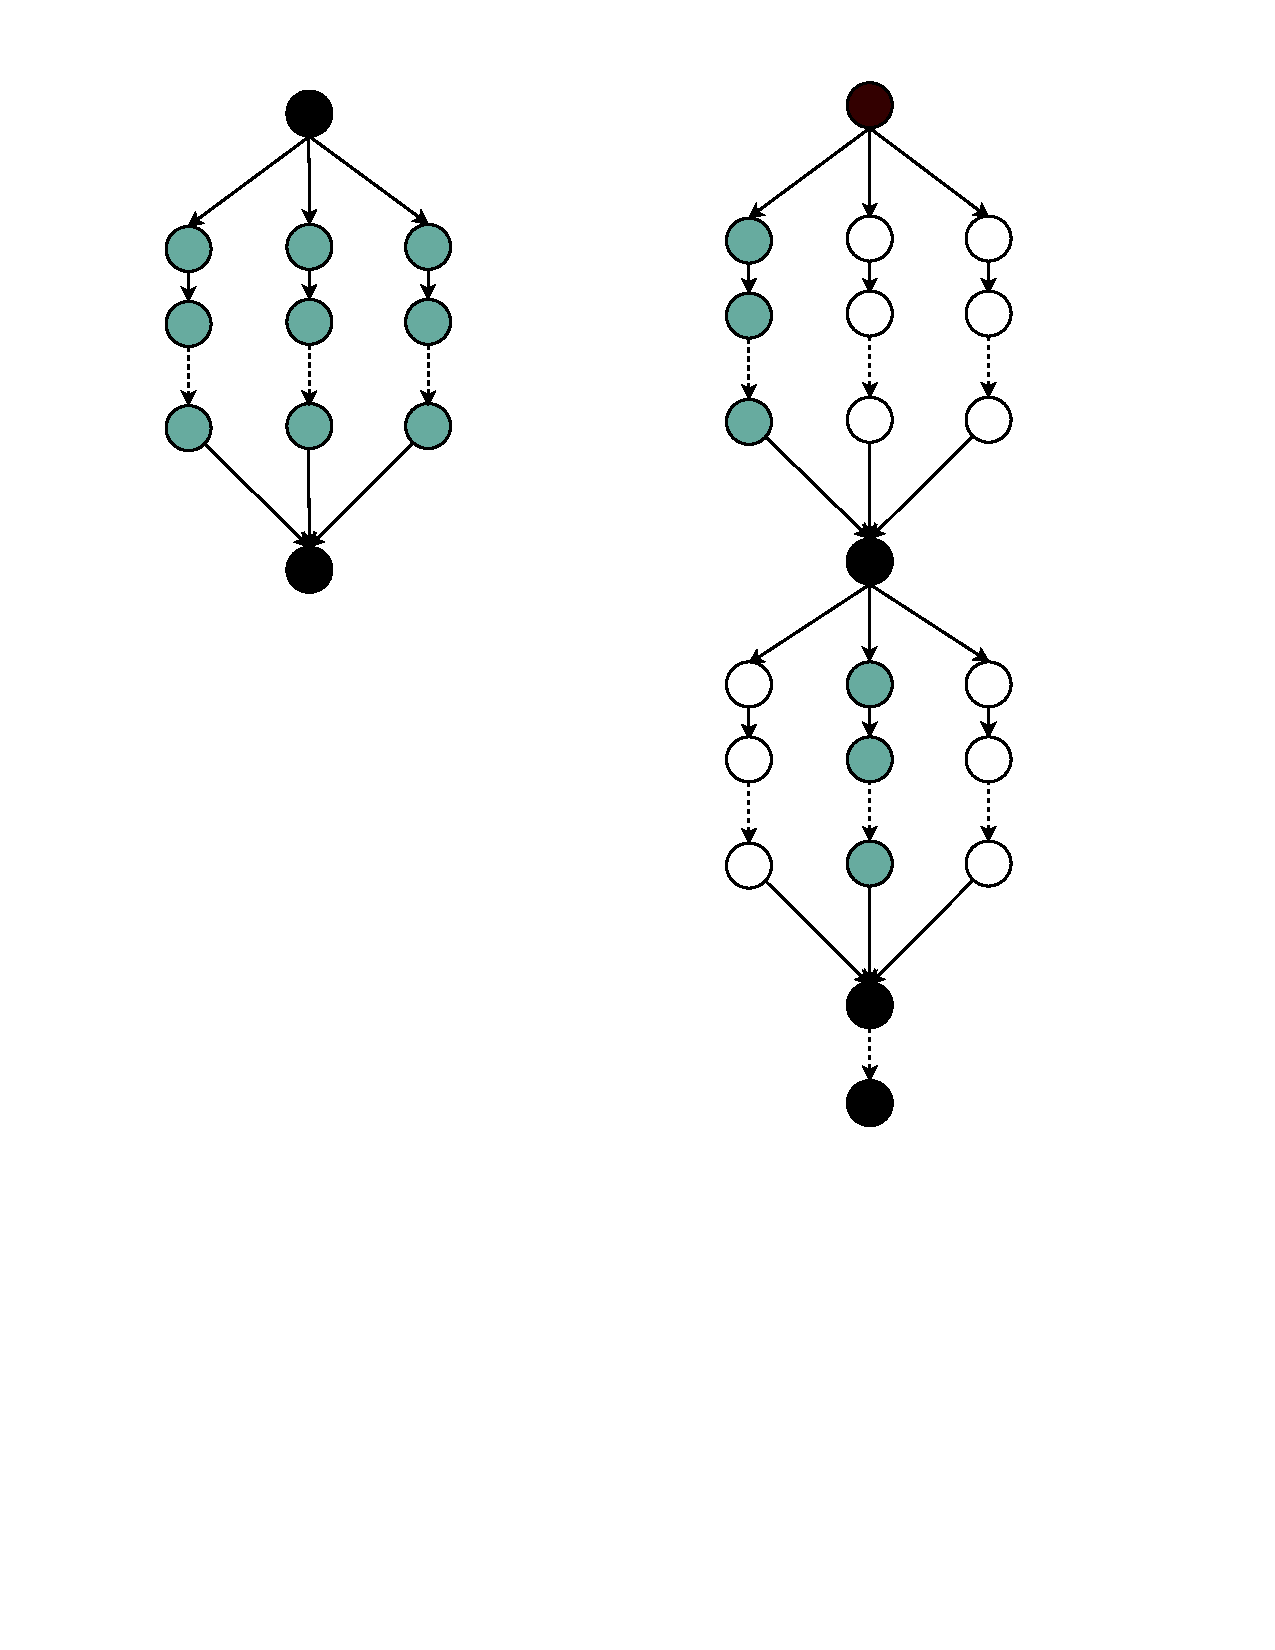
\includegraphics[height=5cm, trim={2.5cm 8cm 4cm 1cm}, clip]{PRAM.pdf}
  \end{center}
  \caption{DAG for PRAM analysis of PPF}
  \label{fig:pram}
\end{figure}

The average parallelism of PPF lies between $O(1)$ and $O(n)$ depending on the input graph. 
In section XY (TODO ref) we show that for real-world input data PPF achieves a speedup that is close to the optimal average parallelism

\subsection{Tree Grafting}\label{sec:tg}

The second algorithm we examined that solves the problem of maximum matching on bipartite graphs is the Tree Grafting algorithm, as described in \cite{Azad:2015}. One of the paper's conclusions is that Tree Grafting performs better over Pothen-Fan on architectures with many thin cores, which the Xeon Phi essentially is. \\
We give a short overview of the algorithm we have implemented and on the optimizations we did.

\mypar{Parallel Tree Grafting} 
Parallel Tree Grafting (PTG) takes a bipartite graph and an initial matching $M $as input and returns a maximum matching by updating $M$.
PTG is - like Pothen-Fan - a multi-source searching algorithm. It starts to search for augmenting paths from different unmatched vertices and constructs a forest of alternating (matched-unmatched) trees.\\
The main difference to Pothen-Fan lies then in the reuse of already found trees. Pothen-Fan forgets about the trees it has previously found and starts again extending the augmenting paths with at most one vertex in every iteration. \\
PTG however keeps track of augmenting trees which can still be extended (active trees) and then grafts other trees to the active trees to prolong the augmenting paths contained in them.\\
For a more detailed explanation of the PTG algorithm including pseudocode, see \cite{Azad:2015}.\\
\mypar{Optimizations}
Our implementation of the PTG algorithm follows the implementation described in the paper very closely. To build the augmenting paths, we have used the same optimizations as already described in our best version of  PPF. To store the pointers to the root, leaf and other nodes the PTG algorithm utilizes, we have implemented our own version of a non-blocking queue as a data structure. 

\section{Experimental Results}\label{sec:exp}

%Here you evaluate your work using experiments. You start again with a
%very short summary of the section. The typical structure follows.

\mypar{Experimental setup} 
%Specify the platform (processor, frequency, maybe OS, maybe cache sizes)
%as well as the compiler, version, and flags used. If your work is about performance, 
%I strongly recommend that you play with optimization flags and consider also icc for additional potential speedup.

Xeon Phi (5110P), GCC, -O3, 60 simplified Intel CPU cores running at 1056 MHz and supports 4 threads per core, resulting in a total of 240 threads. Each core has a 32kb L1 data cache, a 32kb L1 instruction cache and a private 512 kb L2 unified cache. \cite{Ramos:2013}

%Then explain what kind of benchmarks you ran. The idea is to give enough information so the experiments are reproducible by somebody else on his or her code.
%For sorting you would talk about the input sizes. For a tool that performs NUMA optimization, you would specify the programs you ran.
\mypar{Test Data}
To test our algorithms, we have used several graphs from real-world examples. The graphs and their attributes are listed in \ref{table:testdata}. \\
\begin{table}
\centering
\begin{tabular}{ |l|l|l|l| }
\hline
 & $\lvert V \rvert$ & $\lvert E \rvert$ & Density \\ \hline
coPaperDBLP & 1'080'872 & 15'245'732 & $5.22\mathrm{e}{-5}$ \\ \hline
Wikipedia & 7'030'396 & 45'030'392 & $3.64\mathrm{e}{-6}$ \\ \hline
Amazon0312 & 801'454 & 3'200'440 & $1.99\mathrm{e}{-5}$ \\ \hline
Gnutella & 73'364 & 176'656 & $1.31\mathrm{e}{-4}$ \\ \hline
\end{tabular}
\caption{Test data used for benchmarks. $\lvert V \rvert$ is the number of vertices, $\lvert E \rvert$ the number of edges. The density describes the sparseness of the graph, where $0.0$ represents an empty graph and $1.0$ a fully connected bipartite graph.}
\label{table:testdata}
\end{table}
\mypar{Benchmarks}

Sequential Pothen-Fan

\mypar{Verification}

We use the \textit{Edmonds Maximum Cardinality Matching} algorithm \cite{BoostEdmonds} from the Boost Graph library  to verify the correctness of our implementations.

\mypar{Results}
%Next divide the experiments into classes, one paragraph for each. In each class of experiments you typically pursue one questions that then is answered by a suitable plot or plots. For example, first you may want to investigate the performance behavior with changing input size, then how your code compares to external benchmarks.
%
%For some tips on benchmarking including how to create a decent viewgraph see pages 22--27 in \cite{Pueschel:10}.

%{\bf Comments:}
%\begin{itemize}
%\item Create very readable, attractive plots (do 1 column, not 2 column plots
%for this report) with readable font size. However, the font size should also not be too large; typically it is smaller than the text font size.
%An example is in Fig.~\ref{fftperf} (of course you can have a different style).
%\item Every plot answers a question. You state this question and extract the
%answer from the plot in its discussion.
%\item Every plot should be referenced and discussed.
%\end{itemize}
%
%\begin{figure}\centering
%  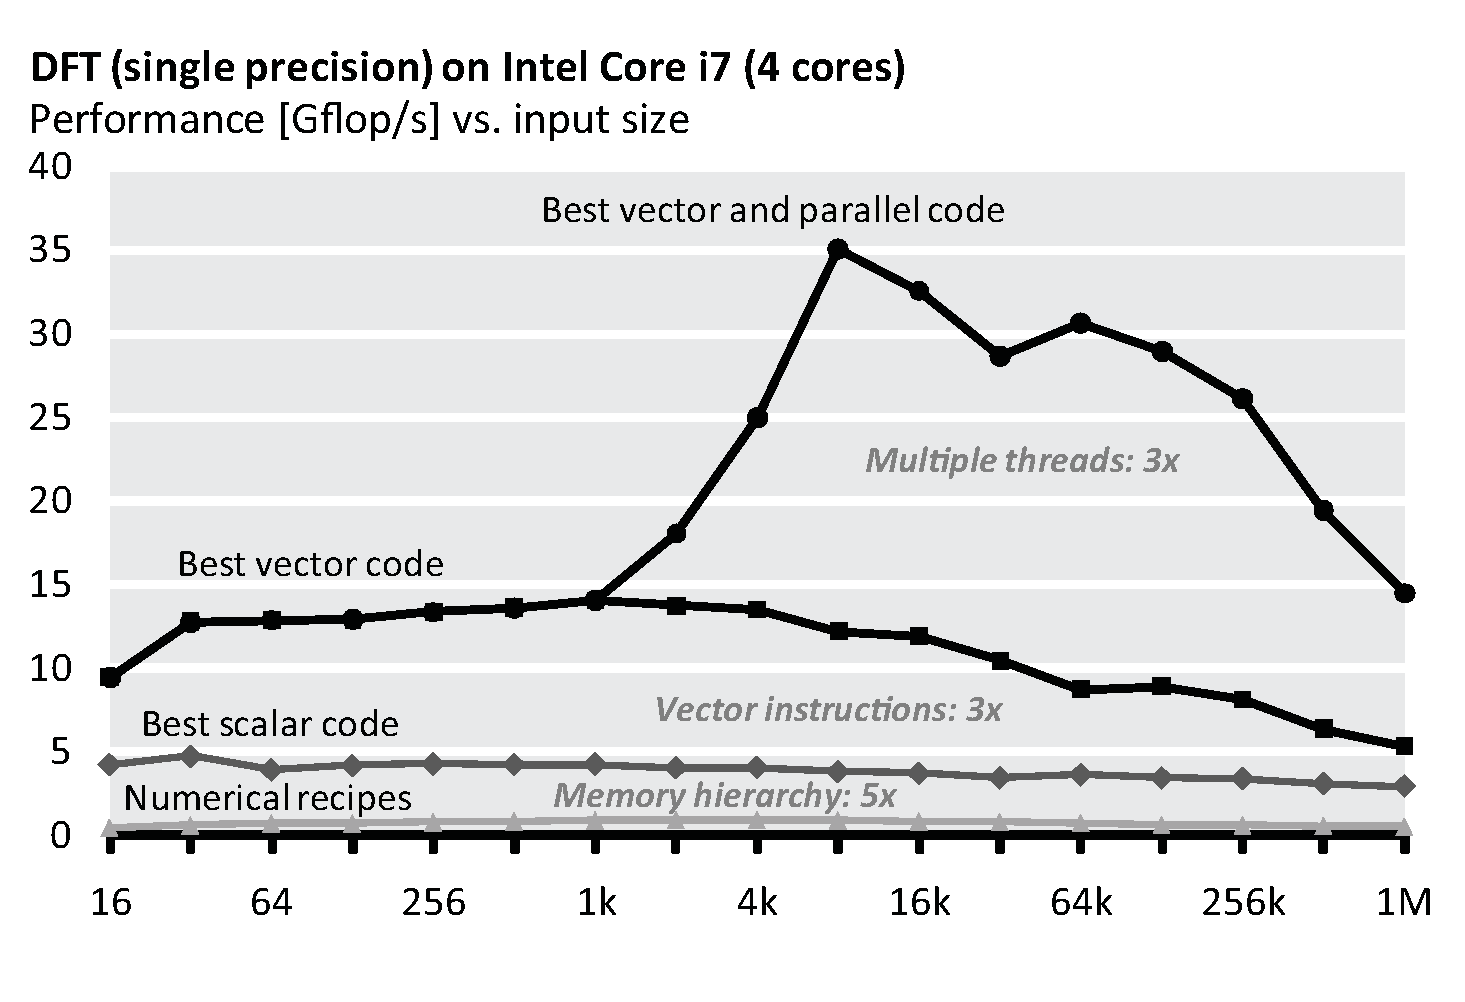
\includegraphics[scale=0.33]{dft-performance.eps}
%  \caption{Performance of four single precision implementations of the
%  discrete Fourier transform. The operations count is roughly the
%  same. The labels in this plot are maybe a little bit too small.\label{fftperf}}
%\end{figure}

\section{Conclusions}

Super linear speedup because of caching effects\\
PPF scales well on Xeon Phi\\
Tree Grafting results from the paper could not be reproduced.
%
%Here you need to summarize what you did and why this is
%important. {\em Do not take the abstract} and put it in the past
%tense. Remember, now the reader has (hopefully) read the report, so it
%is a very different situation from the abstract. Try to highlight
%important results and say the things you really want to get across
%such as high-level statements (e.g., we believe that .... is the right
%approach to .... Even though we only considered x, the
%.... technique should be applicable ....) You can also formulate next
%steps if you want. Be brief. After the conclusions there are only the references.
%
%\section{Further comments}
%
%Here we provide some further tips.
%
%\mypar{Further general guidelines}
%
%\begin{itemize}
%\item For short papers, to save space, I use paragraph titles instead of
%subsections, as shown in the introduction.
%
%\item It is generally a good idea to break sections into such smaller
%units for readability and since it helps you to (visually) structure the story.
%
%\item The above section titles should be adapted to more precisely
%reflect what you do.
%
%\item Each section should be started with a very
%short summary of what the reader can expect in this section. Nothing
%more awkward as when the story starts and one does not know what the direction is or the goal.
%
%\item Make sure you define every acronym you use, no matter how
%convinced you are the reader knows it.
%
%\item Always spell-check before you submit (to us in this case).
%
%\item Be picky. When writing a paper you should always strive for very
%high quality. Many people may read it and the quality makes a big difference.
%In this class, the quality is part of the grade.
%
%\item Books helping you to write better: \cite{Higham:98} and \cite{Strunk:00}.
%
%\item Conversion to pdf (latex users only): 
%
%dvips -o conference.ps -t letter -Ppdf -G0 conference.dvi
%
%and then
%
%ps2pdf conference.ps
%\end{itemize}

%\mypar{Graphics} For plots that are not images {\em never} generate the bitmap formats
%jpeg, gif, bmp, tif. Use eps, which means encapsulate postscript. It is
%scalable since it is a vector graphic description of your graph. E.g.,
%from Matlab, you can export to eps.
%
%The format pdf is also fine for plots (you need pdflatex then), but only if the plot was never before in the format 
%jpeg, gif, bmp, tif.


% References should be produced using the bibtex program from suitable
% BiBTeX files (here: bibl_conf). The IEEEbib.bst bibliography
% style file from IEEE produces unsorted bibliography list.
% -------------------------------------------------------------------------
\bibliographystyle{IEEEbib}
\bibliography{bibl_conf}

\end{document}

